\chapter{Solvent Density Near the Semiconductor Interface During RNEMD Simulations}

In Section 3.3 we utilize MD (specifically, reverse non-equilibrium MD, or RNEMD) simulations to explore the impact of crystal structure and surface passivation in a fully microscopic, atomistic fashion. In particular we note a surprising non-monotonic dependence of interfacial thermal conductance on the extent of surface passivation for crystalline surface presenting a high density of binding sites (namely, the polar $0001$ and $000\bar{1}$ surfaces). In the main text of the chapter, we attribute this turnover to a balance of competing effects: Improved vibrational coupling facilitated by the surface layer improves interfacial thermal conductance significantly (Fig. \ref{f:rnemd4}), although at high surface coverage, the densely packed ligands hinder solvent penetration into the ligand layer, which is necessary for efficient thermal coupling (see Ch. 3 for a complete discussion of this point). The excluded volume effects are quantified as a function of surface coverage in an integrated fashion for the polar surfaces in Figure \ref{f:rnemd6}. In Figure \ref{f:densprof1} below, we present the full ligand and solvent density profiles for each of the surfaces considered in this work. \par

\begin{figure}
\begin{center}
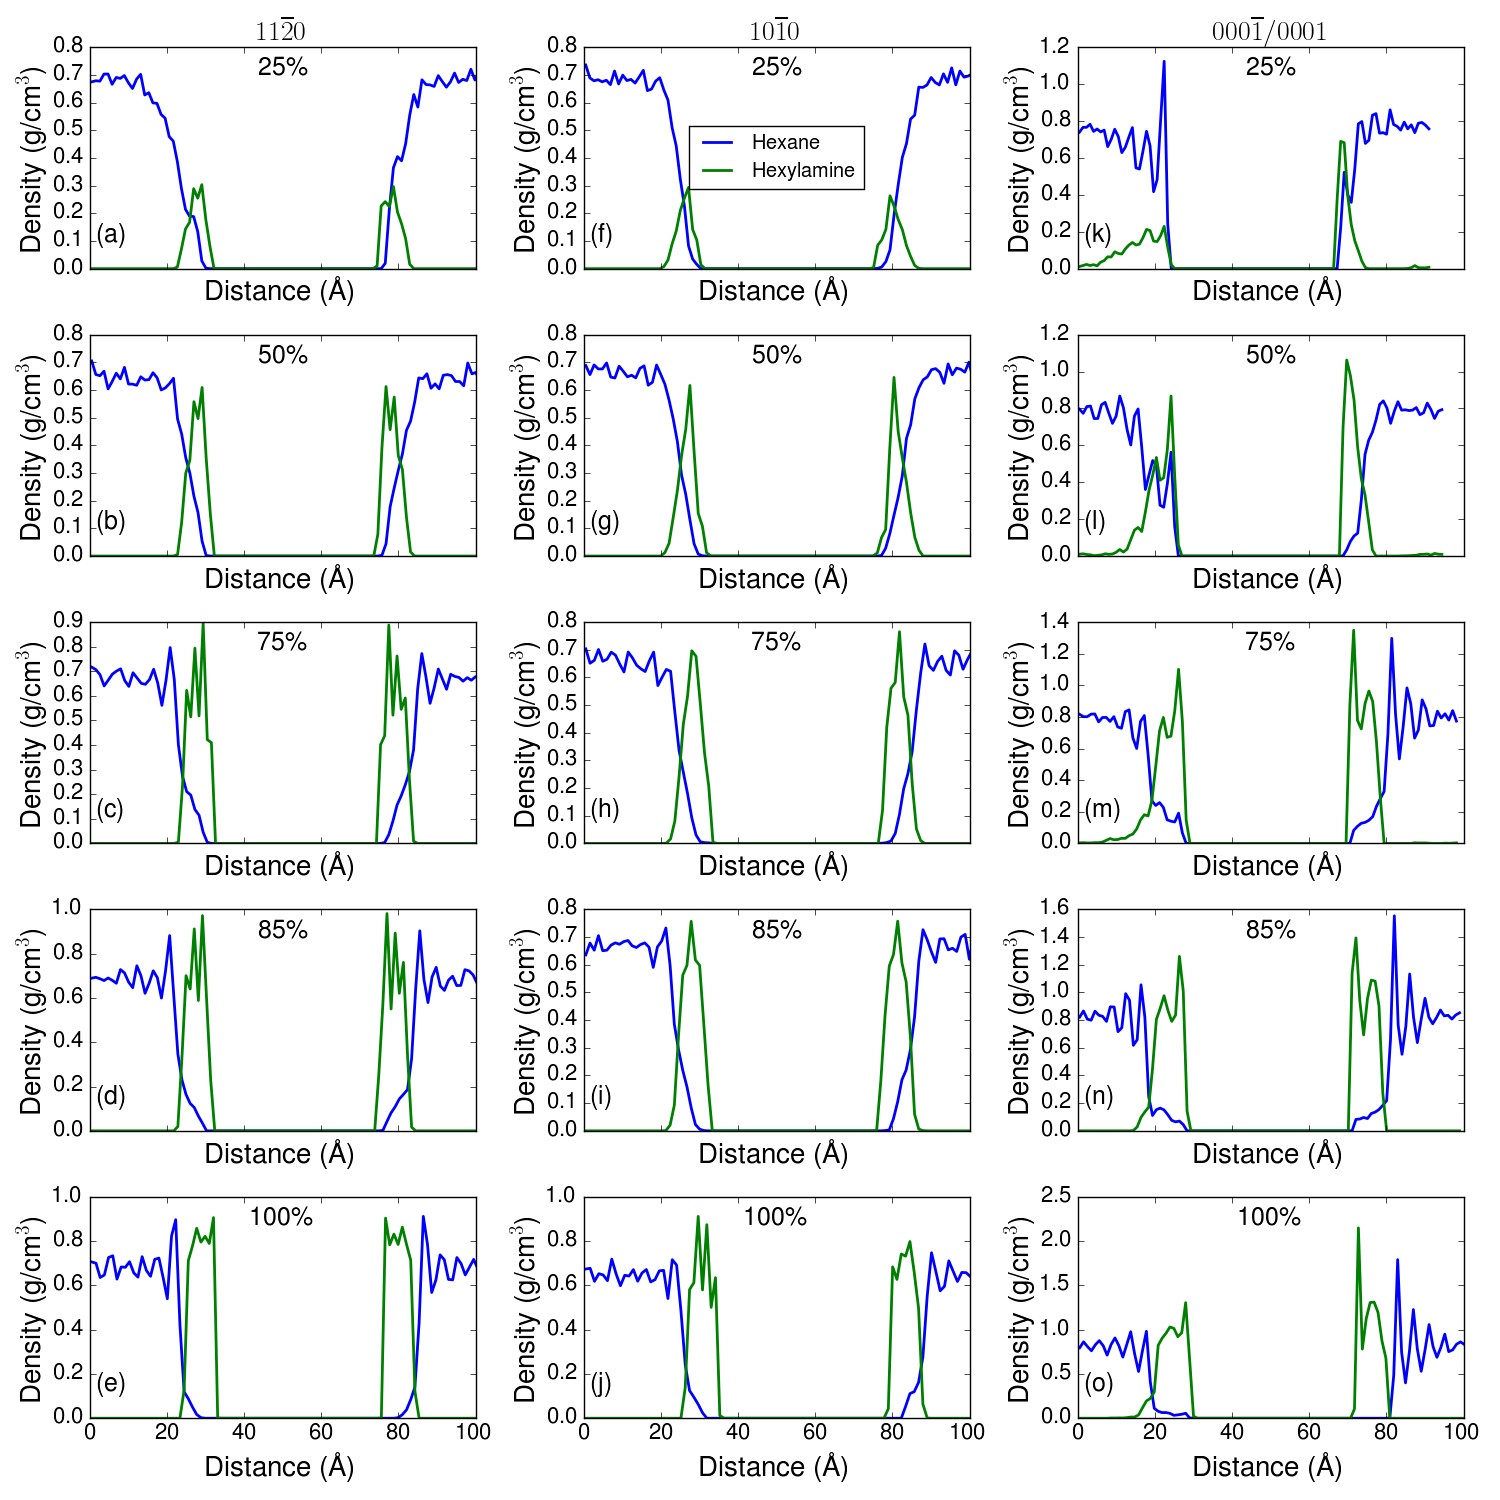
\includegraphics[width=0.75\textwidth]{./appendixE/densprof1.png}
\caption[Ligand and solvent density profiles along the kinetic energy exchange axis for each of the surfaces addressed in Chapter 3 as a function of surface coverage.]{(a) - (o) Density of hexane (blue) and hexylamine (green) molecules along the kinetic energy exchange axis as determined from analysis of RNEMD simulation trajectories susbequent to the development of a stable temperature gradient.}
\label{f:densprof1}
\end{center}
\end{figure}

The profiles shown here were generated subsequent to the development of a stable temperature gradient in RNEMD simulations of the interface beteween liquid hexane and the particular (hexylamine-passivated) exposed CdSe surface. See Chapter 3 for a detailed discussion of the RNEMD methodology. Figure \ref{f:densprof1} highlights the differences in ligand grafting density which are ultimately responsible for the dependence on exposed surface facet. Comparing the 100\% coverage profiles from simulations of the $11\bar{2}0$, $10\bar{1}0$, and $000\bar{1}/0001$ surfaces (Fig. \ref{f:densprof1}(e), (j), and (o), respectively), we note that the solvent density within the ligand layer is is appreciable for the non-polar ($11\bar{2}0$ and $10\bar{1}0$) surfaces, while the more densely passivated polar surfaces exhibit near-complete exclusion of the solvent from the ligand layer. It is this exclusion which lowers interfacial thermal conductance of the 100\%-passivated polar surfaces relative to the 75\% coverage case. These results demonstrate the role played by the structure of the underlying crystalline surface in mediating thermal transport across chemically-passivated interfaces, a previously unexplored concept.


